
[Descrever os produtos a serem gerados, as principais atividades e apresentar um cronograma de trabalho.]

\subsection{Resumo da proposta}
	
	[Escrever um resumo da proposta de trabalho do grupo, responder o que será realizado, qual o ponto de partida e realizar conexões com a fundamentação teórica apresentada.]

\subsection{Estrutura Analítica do Projeto}
	
	[A Estrutura Analítica de Projetos (EAP), do Inglês, Work breakdown structure (WBS) é uma ferramenta de decomposição do trabalho do projeto em partes manejáveis. É estrutura em árvore, hierárquica (de mais geral para mais específica) orientada às entregas que precisam ser feitas para completar um projeto.

	O objetivo de uma WBS é identificar elementos terminais (os produtos, serviços e resultados a serem feitos em um projeto). Assim, a WBS serve como base para a maior parte do planejamento de projeto.
	
	A dica de ferramenta a ser utilizada para elaborar a EAP é o XMIND 
	
	http://www.xmind.net/ ]

\subsection{5.3. Lista de software}
	
	Durante o processo de Avaliação do Sistema Enturma, que engloba desde o Planejamento da Avaliação até a Análise dos Resultados obtidos, serão usados diversos \textit{softwares} e tecnologias para apoiar a Equipe, tais como:

	\begin{itemize}
		\item \textbf{Git}

			O sistema Git será utilizado para Gerência de Configuração e Controle de Versões durante o projeto.

		\item \textbf{GitHub}
			
			Será utilizado como repositório remoto do GIT, para compartilhamento dos dados entre a Equipe.

		\item \textbf{LaTeX}

			Será utilizado para o desenvolvimento de toda a documentação produzida durante a execução deste projeto.

		\item \textbf{Sublime}

			Será utilizado como IDE para o desenvolvimento da Documentação e durante a Evolução do sistema Enturma.

		\item \textbf{GITTER}

			Será utilzado para comunicação, via GitHub, da Equipe durante o Desenvolvimento Projeto.

		\item \textbf{ASES}

			Sistema desenvolvido pelo Governo Federal para Avaliação da Acessibilidade em Sistemas Web.

	\end{itemize}

\subsection{Cronograma de Atividades}

	O Cronograma do Projeto pode ser obtido acessando o link do Drive do Projeto. Como representação, segue a parte inicial do Cronograma de Atividades:

	\begin{figure}[H]
		\centering
		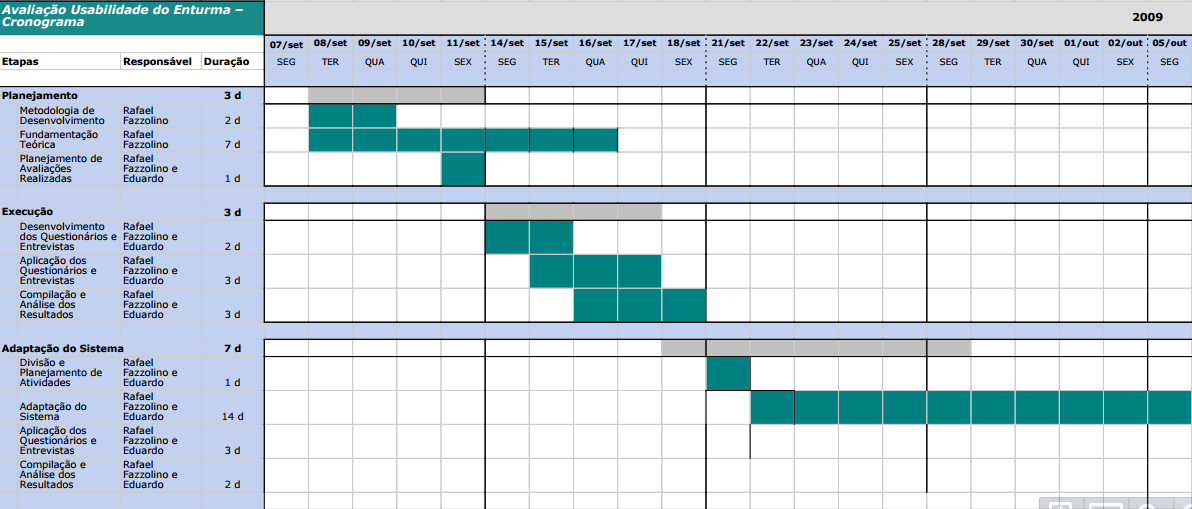
\includegraphics[width=1\textwidth]{imagens/cronograma}
		\caption{Cronograma Inicial do Projeto}
		\label{img:cronograma}
	\end{figure}

